\documentclass[aspectratio=169]{beamer}
\usepackage[utf8]{inputenc}
\usepackage{hyperref}
\usepackage{amsmath,amsfonts,amsthm,bm}
\usepackage{color}
\usepackage{minted}
\usepackage{graphicx} % Allows including images
\usepackage{booktabs} % Allows the use of \toprule, \midrule and \bottomrule in tables
\usepackage{tikz}
\usepackage{mhchem}
\usepackage{pgfplots}

\setminted{fontsize=\scriptsize}

\hypersetup{
    colorlinks=true,
    linkcolor=red,
    filecolor=magenta,      
    urlcolor=red,
}

\DeclareMathOperator*{\argmax}{argmax}
\DeclareMathOperator*{\argmin}{argmin}
\let \vec \mathbf

\mode<presentation> {
    \usetheme{CambridgeUS}
    %\setbeamertemplate{footline} % To remove the footer line in all slides uncomment this line
    \setbeamertemplate{footline}[page number] % To replace the footer line in all slides with a simple slide count uncomment this line
    \setbeamertemplate{navigation symbols}{} % To remove the navigation symbols from the bottom of all slides uncomment this line
}


\title[Linear Classification]{Linear Classification}

\author{Shyue Ping Ong}
\institute[UCSD]{University of California, San Diego\\
\medskip
}
\date{NANO281} % Date, can be changed to a custom date

\begin{document}


\begin{frame}
    \titlepage % Print the title page as the first slide
\end{frame}


\begin{frame}{Overview}
    \tableofcontents
\end{frame}


\section{Preliminaries}

\begin{frame}{Preliminaries}
    \begin{itemize}
        \item Linear methods can also be used for classification, i.e., decision boundaries are linear.
        \item These methods are surprisingly effective across a large spectrum of datasets, even compared to more complex ML models.
    \end{itemize}
\end{frame}


\begin{frame}{Metal vs Insulator Dataset}
    \begin{itemize}
        \item To demonstrate the use of these methods, we will first discuss the ``toy'' dataset.
        \item 2000+ binary (\ce{A_xB_y}) compounds with experimental band gaps.
        \item Class 0: metals; Class 1: insulators.
        \item Using pymatgen, we can generate some simple features. Here, we will create simply features based on the mean and absolute difference in electronegativity between A and B (why?).
    \end{itemize}
    \begin{figure}
        \centering
        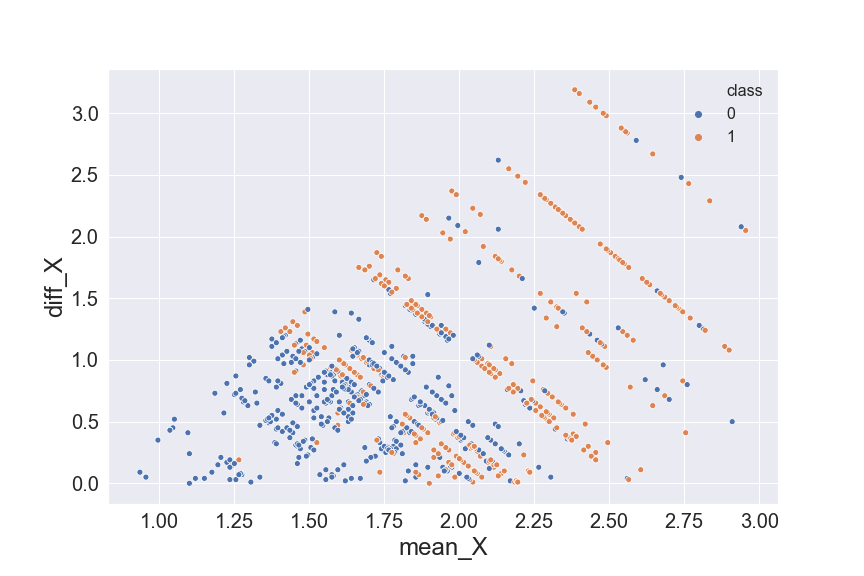
\includegraphics[width=0.5\textwidth]{figures/electronnegativity_bandgap.png}
    \end{figure}
\end{frame}


\begin{frame}[fragile]{Creating the features and classes}
\begin{minted}{python}
import pandas as pd
from pymatgen import Composition
binaries = pd.read_csv('binary_band_gap.csv')
# We create a column holding the Composition object. 
# Note the use of list comprehension in Python.
binaries['composition'] = [Composition(c) for c in binaries['Formula']]
electronegs = [[el.X for el in c] for c in binaries['composition']]
# Create the features mean and difference between electronegativities
binaries['mean_X'] = [np.mean(e) for e in electronegs]
binaries['diff_X'] = [max(e) - min(e) for e in electronegs]
# Label metals (band gap of 0. 1e-5 is used as numerical tolerance) as class 0
# Insulators are labelled as class 1.
binaries['class'] = [0 if eg < 1e-5 else 1 for eg in binaries['Eg (eV)']]}
\end{minted}
\end{frame} 


\section{Basic concepts}

\begin{frame}{Basic concepts}
    \begin{itemize}
        \item If there are $K$ classes, we have a $N \times K$ indicator response matrix. Each row is a vector $Y = (Y_1, Y_2, ..., Y_K)$ where $Y_k = 1$ if the instance belongs to the $k$th class and all other $Y$s are 0.
        \begin{equation*}
            \vec{Y} = \begin{pmatrix}
            0 & 0 & ... & 1\\
            1 & 0 & ... & 0\\
            ...& & &\\
            0 & 1 & ... & 0\\
            \end{pmatrix}
        \end{equation*}
        \item For the $k$th response variable, the fitted $\hat{f_k}(x) = \hat{\beta_{k0}} + \hat{\beta_{k}^T}x$.
        \item Decision boundary between $k$ and $l$ class is given by $\hat{f_k}(x) = \hat{f_l}(x)$. 
        \item Input is divided into regions.
        \item Similar to linear regression, we can augment the input space with polynomial (e.g., $X_1^2, X_2^s, X_1X_2$) and other basis functions, leading to boundaries that are non-linear.
    \end{itemize}
\end{frame} 


\begin{frame}
\frametitle{Linear regression of indicator matrix}
\begin{columns}
\column{0.5\textwidth}
    \begin{itemize}
        \item Treat each column of $\vec{Y}$ as a target. Least squares solution:
        \begin{equation*}
            \hat{\vec{Y}} = \vec{X}(\vec{X}^T\vec{X})^{-1}\vec{X}^T\vec{Y}
        \end{equation*}
        \item For each new observation $x$, we compute $\hat{f_k}(x) = (1, x^T)(\vec{X}^T\vec{X})^{-1}\vec{X}^T\vec{Y}$.
        \item Find the largest component, and that will result in the classification k, $G(x) = \argmax_{k \in G} \hat{f_k}(x)$.
        \item Major issue: some categories may be masked for $K \geq 3$.
    \end{itemize}
\column{0.5\textwidth}
    \begin{figure}
        \centering
        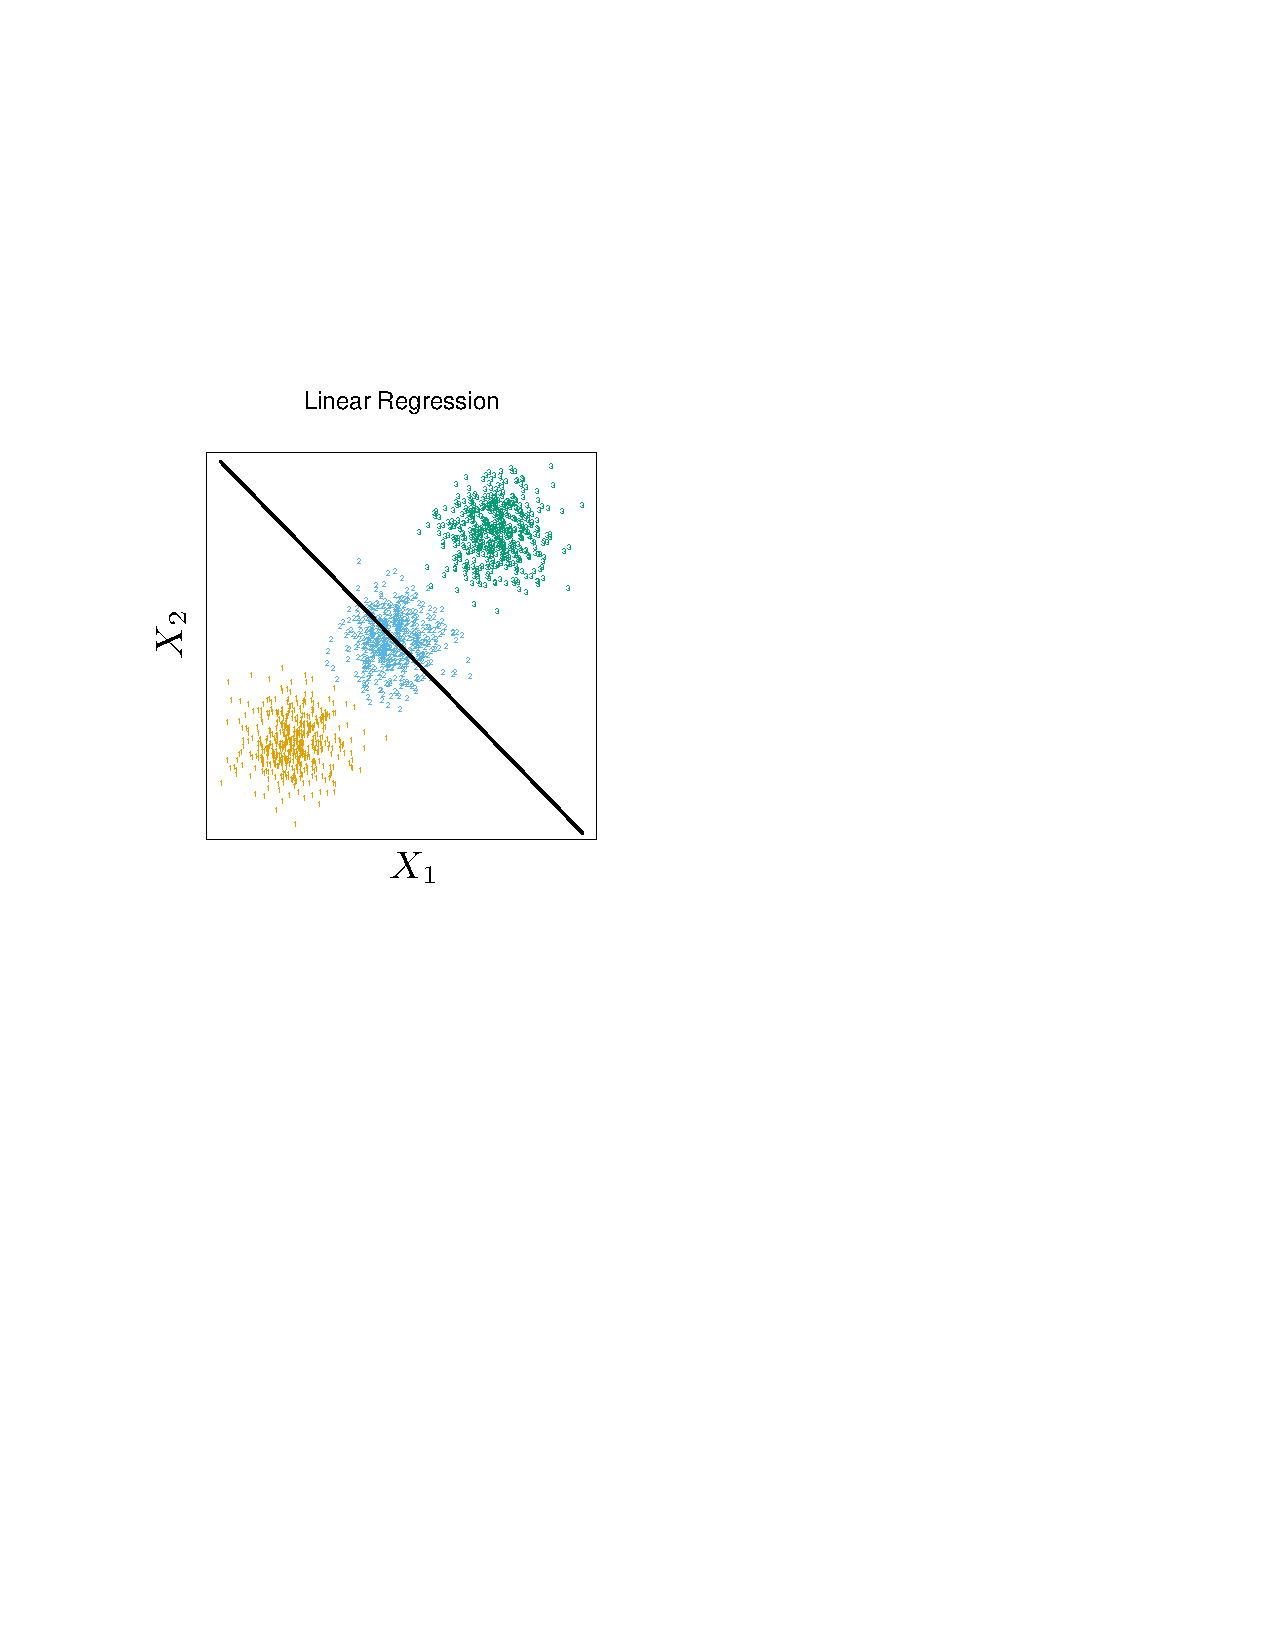
\includegraphics[width=0.8\textwidth]{figures/linearclassifier.pdf}
    \end{figure}
\end{columns}
\end{frame} 


\section{Discriminant Analysis}

\begin{frame}{Discriminant Analysis}
    \begin{itemize}
        \item From Bayes rule, we have:
        \begin{equation*}
            P(G = k|X = x) = \frac{f_k(x)\pi_k}{\sum_{l=1}^K f_l(x)\pi_l}
        \end{equation*}
        \item where $f_k(x)$ are the class conditional probability densities ($P(X = x | G=k)$) and $\pi_k$ are the prior probabilities of being in class $k$.
        \item Most common approach - assume Gaussian class densities.
        \begin{equation*}
            f_k(x) = \frac{1}{(2\pi)^{p/2}|\Sigma_k|^{1/2}}\exp{-\frac{1}{2}(x-\mu_k)^T\Sigma_k^{-1}(x-\mu_k)}
        \end{equation*}
    \end{itemize}
\end{frame} 


\begin{frame}{Linear Discriminant Analysis}
    \begin{itemize}
        \item Assume all classes have a common covariance matrix, i.e., $\Sigma_k = \Sigma$.
        \item To compare two classes $k$ and $l$, we can compare the log ratios.
        \begin{eqnarray*}
            \log{\frac{P(G = k|X = x)}{P(G = l|X = x)}} & = & \log{\frac{f_k(x)}{f_l(x)}} + \log{\frac{\pi_k}{\pi_l}}\\
            & = & \log{\frac{\pi_k}{\pi_l}} -\frac{1}{2}(\mu_k+\mu_l)^T\Sigma^{-1}(\mu_k-\mu_l) \\
            & & + x^T \Sigma^{-1} (\mu_k - \mu_l)
        \end{eqnarray*}
        \item At the decision boundary, $P(G=k|X=x) = P(G=l|X=x)$, which leads to a linear equation in $x$.
        \item Equivalently, we have
        \begin{equation*}
            G(x) = \argmax_k \left \{ \log{\pi_k} -\frac{1}{2}\mu_k^T\Sigma^{-1}\mu_k + x^T \Sigma^{-1} \mu_k \right \}
        \end{equation*}
    \end{itemize}
\end{frame}


\begin{frame}{Linear Discriminant Analysis, contd.}
    \begin{itemize}
        \item In general, we do not know the prior distributions and covariance matrix. These are estimated from the data.
        \begin{itemize}
            \item $\hat{\pi_k} = N_k/N$
            \item $\hat{\mu_k} = \sum_{g_i=k} x_i / N$
            \item $\hat{\Sigma} = \sum_{k=1}^K \sum_{g_i=k} (x_i - \hat{\mu_k})^T(x_i - \hat{\mu_k}) / (N - K)$
        \end{itemize}
        \item Avoids masking problem of linear regression classification.
        \item For the example data,
        \begin{figure}
            \centering
            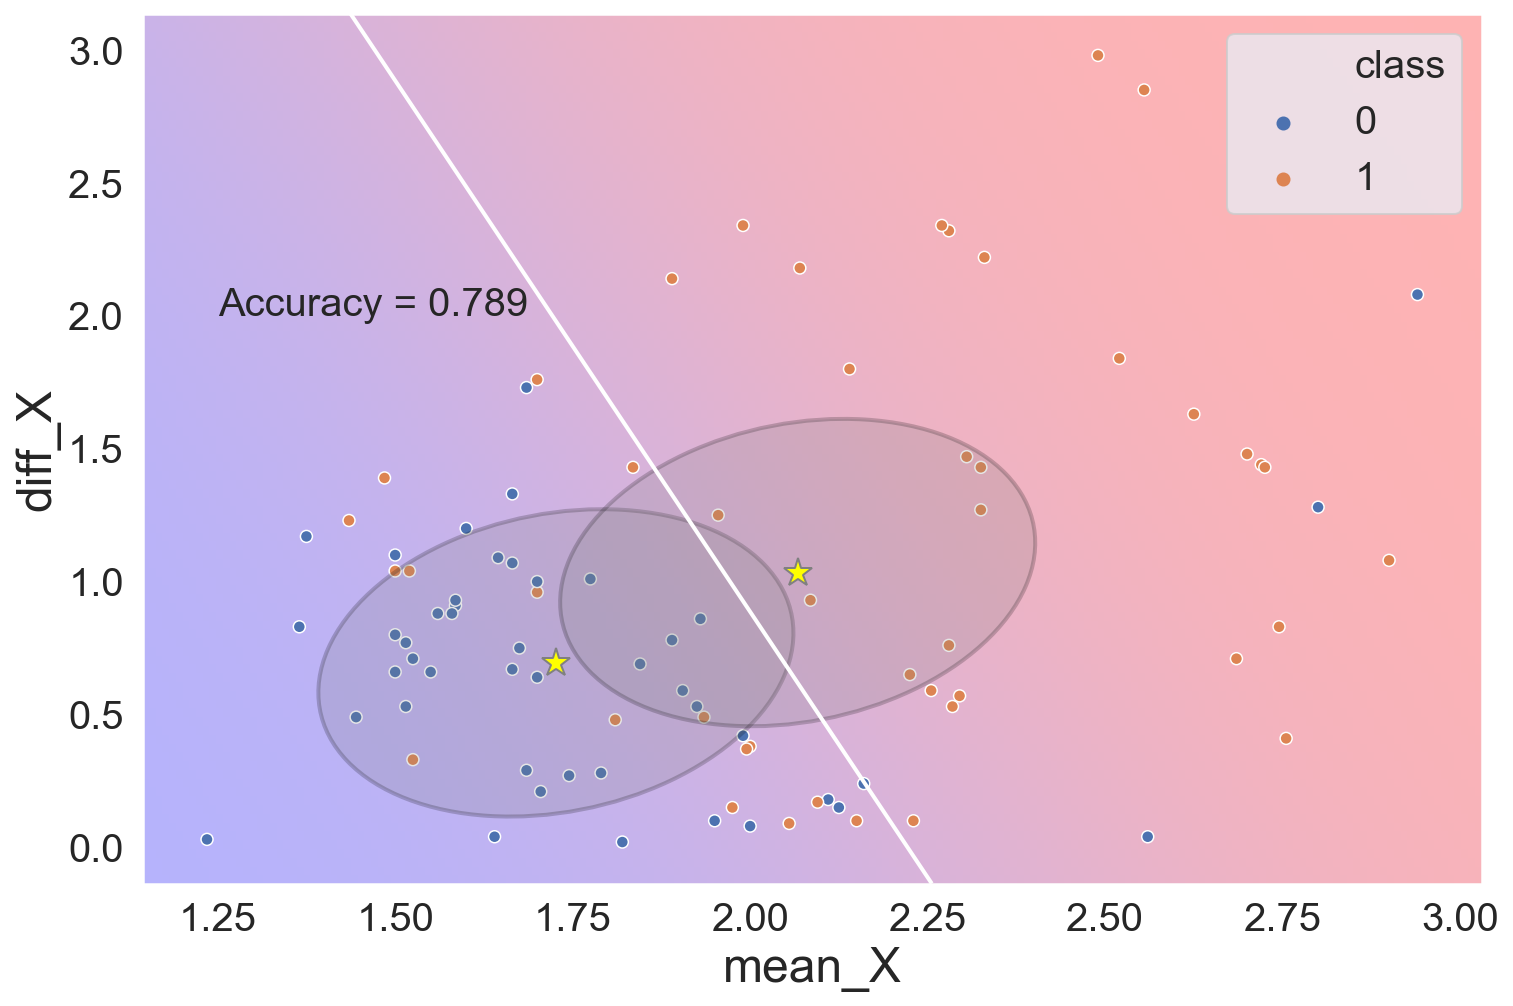
\includegraphics[width=0.5\textwidth]{figures/lda_metal_insulator.png}
        \end{figure}
    \end{itemize}
\end{frame}


\begin{frame}{Quadratic Discriminant Analysis}
    \begin{itemize}
        \item Covariances are not assumed equal.
        \begin{equation*}
            G(x) = \argmax_k \left \{ \log{\pi_k} -\frac{1}{2}(x-\mu_k)^T\Sigma_k^{-1}(x-\mu_k) -\frac{1}{2} \log{|\Sigma_k|} \right \}
        \end{equation*}
        \item No cancellation of terms and decision boundaries are quadratic.
        \item Covariances must be estimated for each category.
        \item For the same metal-insulator example,
        \begin{figure}
            \centering
            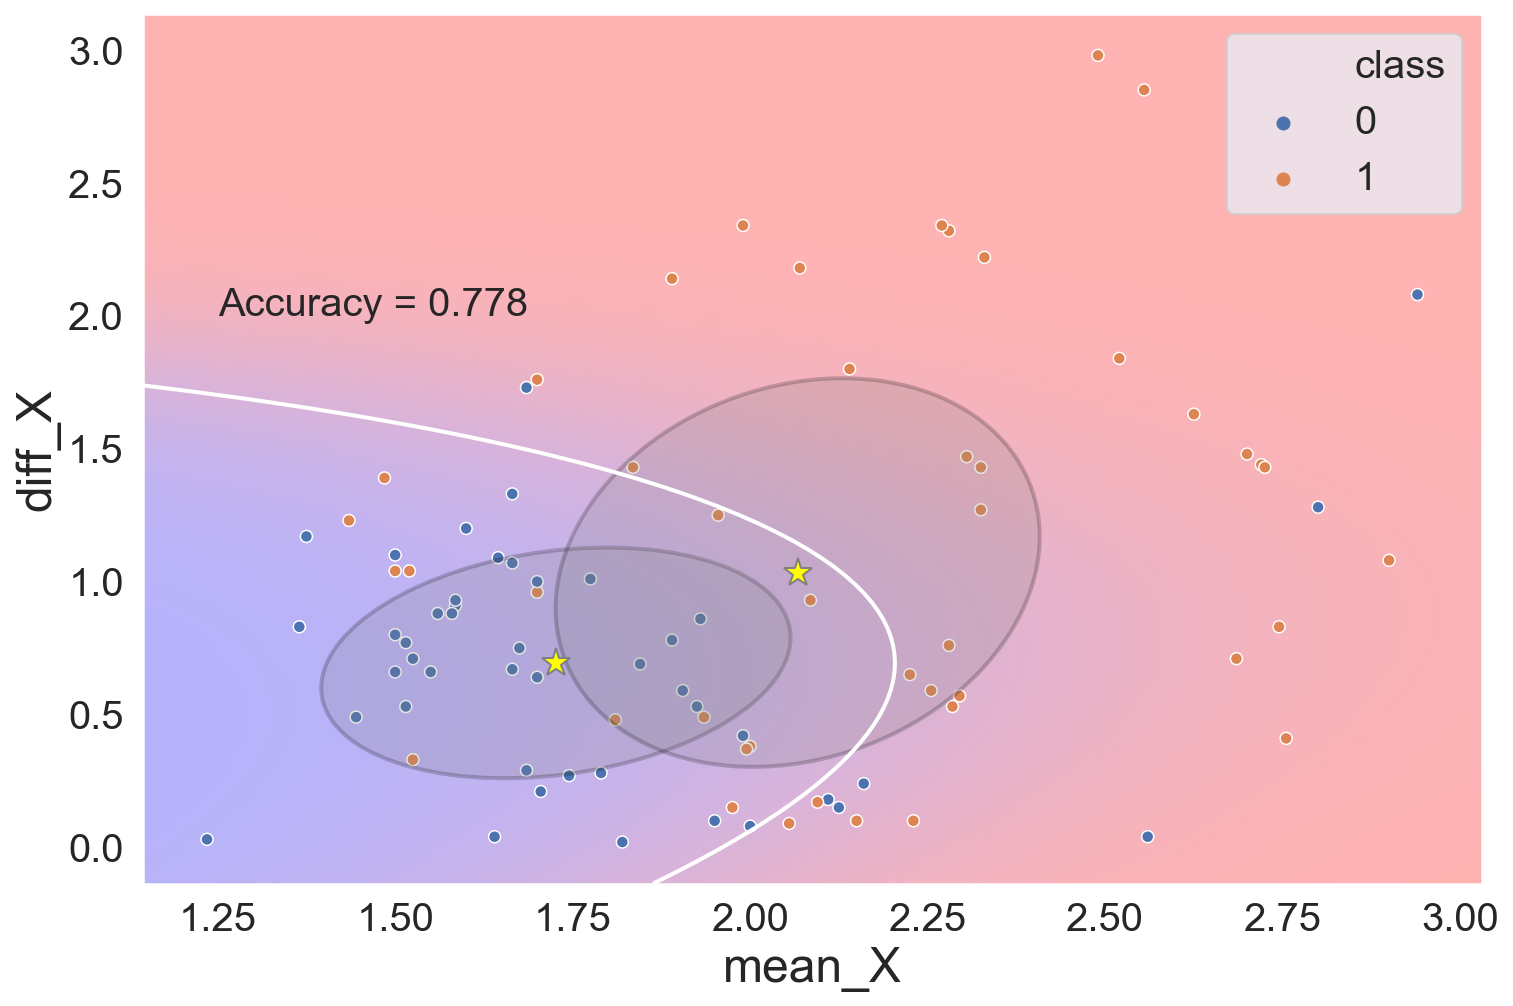
\includegraphics[width=0.5\textwidth]{figures/qda_metal_insulator.png}
        \end{figure}
    \end{itemize}
\end{frame}


\begin{frame}[fragile]{Discriminant analysis in scikit-learn}
\begin{minted}{python}
from sklearn.discriminant_analysis import LinearDiscriminantAnalysis,
    QuadraticDiscriminantAnalysis
lda = LinearDiscriminantAnalysis(solver="svd", store_covariance=True)
X = binaries[["mean_X", "diff_X"]]
y = binaries["class"]
model = lda.fit(X, y)
y_pred = model.predict(X)

qda = QuadraticDiscriminantAnalysis(store_covariance=True)
y_pred = qda.fit(X, y).predict(X)
\end{minted}
\end{frame} 


\begin{frame}{Logistic regression}
    \begin{itemize}
        \item Model posterior probabilities with linear function.
        \begin{eqnarray*}
            \log{\frac{P(G=1|X=x)}{P(G=K|X=x)}} & = & \beta_{10} + \beta_1^T x\\
            \log{\frac{P(G=2|X=x)}{P(G=K|X=x)}} & = & \beta_{20} + \beta_2^T x\\
            & ... &\\
            \log{\frac{P(G=K-1|X=x)}{P(G=K|X=x)}} & = & \beta_{(k-1)0} + \beta_{k-1}^T x\\
        \end{eqnarray*}
        \item Results in the following posterior probabilities:
        \begin{eqnarray*}
            P(G=1|X=x) & = & \frac{\exp{(\beta_{10} + \beta_1^T x)}}{1 + \sum_{l=1}^{K-1}\exp{(\beta_{l0} + \beta_l^T x})}\\
            P(G=K|X=x) & = & \frac{1}{1 + \sum_{l=1}^{K-1}\exp{(\beta_{l0} + \beta_l^T x})}\\
        \end{eqnarray*}
    \end{itemize}
\end{frame} 


\begin{frame}{Solving for the Logistic Regression Coefficients}
    \begin{itemize}
        \item Typically fitted using \textit{maximum likelihood}.
        \begin{equation*}
            l(\beta) = \sum_{i=1}^N \log {P(G = k | X = x i; \beta)}
        \end{equation*}
        \item Differentiation and setting $\frac{\partial{l}}{\partial{\beta}} = 0$ leads to equations that are non-linear in $\beta$.
        \item These equations are solved using some optimization algorithm (e.g., Newton-Raphson, BFGS, etc.). 
    \end{itemize}
\end{frame} 


\begin{frame}[fragile]{Logistic regression on metal/insulator dataset}
\begin{minted}{python}
from sklearn.linear_model import LogisticRegression
clf = LogisticRegression(penalty='none', random_state=0)
model = clf.fit(X, y)
y_pred = model.predict(X)
\end{minted}
\begin{figure}
    \centering
    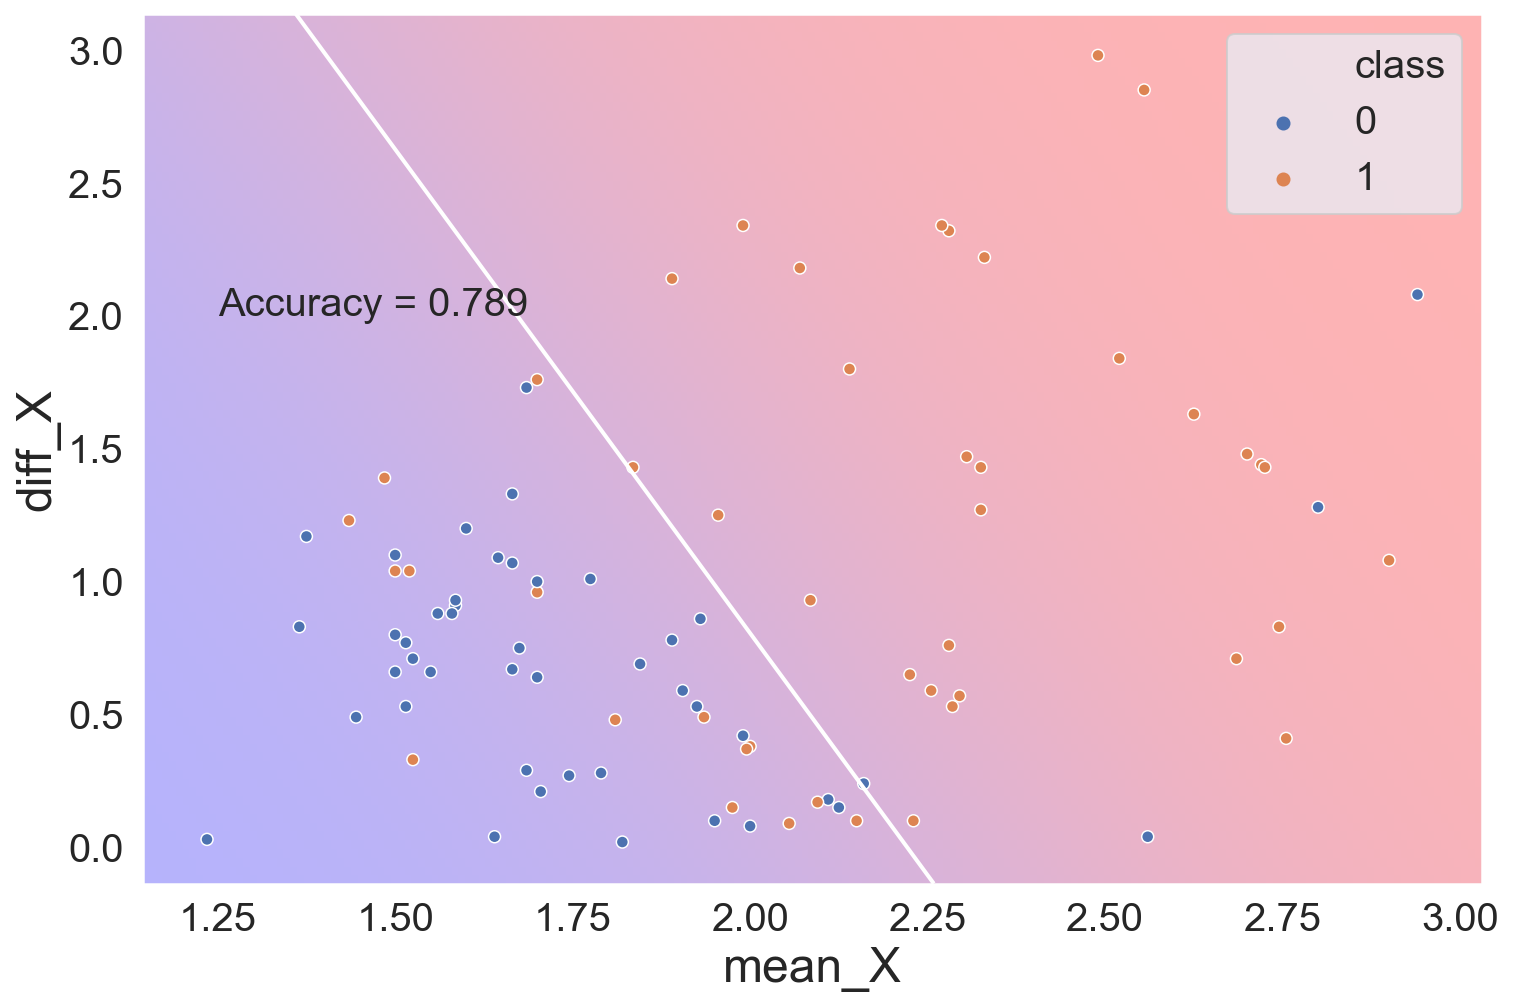
\includegraphics[width=0.8\textwidth]{figures/logistic_metal_insulator.png}
\end{figure}
\end{frame} 


\begin{frame}{Bibliography}
    \bibliographystyle{unsrt}
    \bibliography{refs}
\end{frame}


\begin{frame}
    \Huge{\centerline{The End}}
\end{frame}

\end{document}

